\documentclass[12pt]{scrartcl}
\input{C:/Users/Nia/Documents/Hobbies/Mathematics/Typesetting/nia_defs.tex}
\parskip=0.5cm

\title{\vspace{-2em}Types, Print, and If Review}
\author{}
\date{}

\begin{document}
\maketitle
\vspace{-6em}

\section{Installation and Using Python}
\subsubsection*{Installing Python}
You can install Python by heading to its \href{https://www.python.org/}{website}. Just make sure you have the appropiate version for your operating system (Windows, Mac, Etc.), and \textbf{if on Windows, check ``Add to Path''} on the first screen of the installer. This allows you to run Python code on any folder in your computer!

To check if Python installed right, you can open Command Prompt on Windows by typing \codel{cmd} in your Windows Search Bar in the bottom left corner. Then, inside the black box that opens, type \codel{python} and press enter. You should get a version number if installation was a success! Then type \codel{quit()} to leave this version number screen.

\begin{figure}[H]
    \centering
    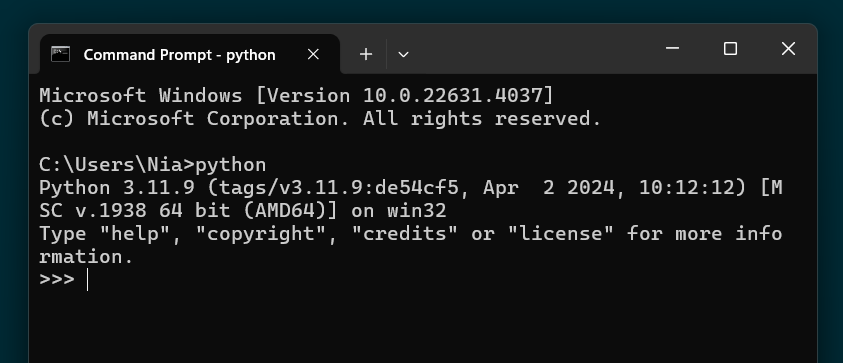
\includegraphics[scale=0.6]{Successful Installation.png}
    \caption*{Successful Installation!}
\end{figure}

We'll be using command prompt a lot, so you'll have plenty of time to become more comfortable with it. Think of command prompt as the ability for us programmers to get closer to the computer than the average person needs to.
    
\subsubsection*{Installing a Text Editor}
Next, you'll need a text editor to write code in. Think of a text editor as google docs or Microsoft Word but for code. You use a text editor for writing code as they have handy features like highlighting your code in different colors to make it easier to read. For beginners, I recommend SublimeText, which you can install \href{https://www.sublimetext.com/}{here}.

\begin{figure}[H]
    \centering
    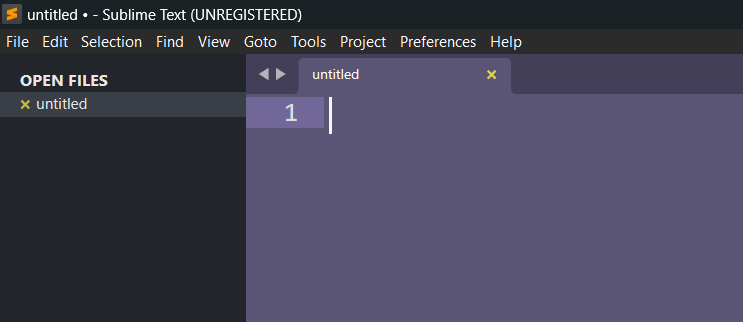
\includegraphics[scale=0.6]{Sublime.png}
    \caption*{Yours will be a different color as I have a theme.}
\end{figure}

\subsubsection*{Running Python Code}
Create a new Python file in Sublime Text by, via the top left menu, click\\ \codel{File $\to$ New File}. When naming your file, \textbf{you can pick any name so long as you end it with} \codel{.py}. This is what tells your computer you are creating a Python file.

Next, you want to navigate via command prompt to the folder you saved your empty Python file in. Remember you can open command prompt by typing ``cmd'' in the Window's search bar in the bottom left corner. In command proompt, you can enter a folder with the command \codel{cd <folder name>}, which stands for change directory. Directory is another word for a folder on computers. If you make a mistake, you can type \codel{cd ..}  to head outwards. See the following example.

\begin{figure}[H]
    \centering
    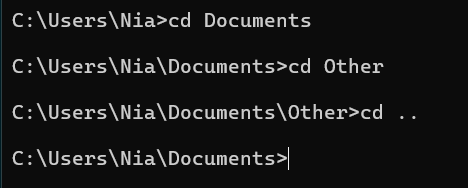
\includegraphics[scale=0.7]{Change Directory.png}
    \caption*{Notice how I used \codel{cd ..} to exit my folder \codel{Other}.}
\end{figure}

If you named your program \codel{FirstProgram.py} and you navigated command prompt to the correct folder, then typing \codel{python FirstProgram.py} in command prompt and pressing enter will run your prgraom! In Sublime Text, write a simple program like this:
\begin{python}
print("Hello World!")
\end{python}
And you'll find ``Hello World!'' on the screen in command prompt when you run your program! Try changing ``Hello World'' to other things in Sublime Text and see them be printed in command prompt.For example, you could replace ``World'' with your name.

\section{Assignment Operator}
Consider this Python code:
\begin{python}
    a = 5
    a = a + 2
    print(a)
\end{python}
What will show up in command prompt? \codel{a}? \codel{5}? Or maybe \codel{7}? Run it yourself.

The answer is indeed 7, as we set $a$ to 5 and then added 2 to it. But hold on. If we think about what this code means from an algebra perspective, aren't we saying:
\begin{align*}
    a &= a + 2 \\
    -a&\quad-a \\
    0 &= 2 \quad \text{(???)}
\end{align*}

In programing, the equal sign $=$ is called the assignment operator. We're not saying that $a$ is equal to $a+2.$ Rather,  we're saying that the variable $a$ should change its value to what it was before plus 2. $a$ was not equal to $a+2$ before, but it will be now. You can think of it like we're crossing out $5$ in memory and replacing it with a 7. I like to say programming is like math that happens over time, so variables can change their values.

Fun Fact: To differentiate the assignment operator $=$ from the equal sign in math, some programming languages use $:=$ instead, which is called the Walrus operator because it looks like Walrus teeth.

\section{Data Types}
In our first lesson, we talked about a few data types. They were:
\begin{itemize}
    \item \pythonl{int} - For holding integers. Example: \pythonl{a = 5}. if you wrote a program \pythonl{print(type(a))}, you will have \pythonl{int} pop up in command prompt when you run the program.
    \item \pythonl{float} - For holding decimal numbers. Example: \pythonl{a = 2.3}. It's called \pythonl{float} partly because when you multiply a decimal number by 10, like $5.2 \cdot 10$, the decimal ``moves over''.
    \item \pythonl{str} - For holding English words. Example: \pythonl{b = "dinosaur"}. \pythonl{str} is short for string, which means a string of characters in a row. Remember that your computer will have an error for \pythonl{a = 5 + "7"} because \pythonl{"7"} is the key 7 on your keyboard, not the number, so you're trying to add a number to text! It would be like \pythonl{a = "banana" + 23}.
    \item \pythonl{bool} - For \pythonl{True} and \pythonl{False}. Example: \pythonl{a = True}. Short for boolean, and named after George Bool who invented using True and False for logic. Bools are really useful for if-statements, which I'll review in the next section.
\end{itemize}

\section{If Statements}
What if you want code to only run some of the time? That's where if-statements come in handy! Consider this code:
\begin{python}
    a = True
    if a:
        print("Success!")
    else:
        print("Not Success.")
\end{python}
If you ran this program in command prompt, would ``Success!'' be printed or ``Not Success''? The answer is ``Success'' because the top part of an if-statement happens only if the \textbf{condition}, which in this case is $a$, is true. Otherwise, the \pythonl{else} section will run.

What about for this program?
\begin{python}
    a = 8
    if a == 19:
        print("Success!")
    else:
        print("Not Success.")
\end{python}
Because we use $=$ for the assignment operator in Python, which is setting a variable to some value, to check if a variable is equal to something, we use $==$ in programming. Here, because $8$ is not eqaul to 19, ``Not Success'' will be printed.

\section{Optional Homework}
Create a folder on your computer called \codel{If-Statements-Practice-1}. Using Sublime Text's new file feature, create multiple python programs that do the following:
\begin{enumerate}
    \item Print the numbers 1 through 5. There's a quick way to do this you'll learn in the future, but for now, just write 5 print statements, 1 for each number.
    \item Sets \pythonl{a = "cat"}, and then print \pythonl{True} if $a$ is a string. Remember that \pythonl{type(a)} is how you check the type of the variable $a$.
    \item Prints the result of $2 + 6.$ Your answer should not be \pythonl{print(8)} but instead should use $2$ and $6.$
\end{enumerate}

Good luck! If you aren't able to finish any of these 3, that's okay; we can talk about them next time.
\end{document}